% Name: Torque on a lever arm
% Description: A force F applied at distance r from a pivot at angle φ to the arm: its parts along and across the arm, the moment arm r sin φ, and the torque it produces.
% Tags: torque, moment, lever arm, rotation

\usetikzlibrary{arrows.meta, angles, quotes, calc}

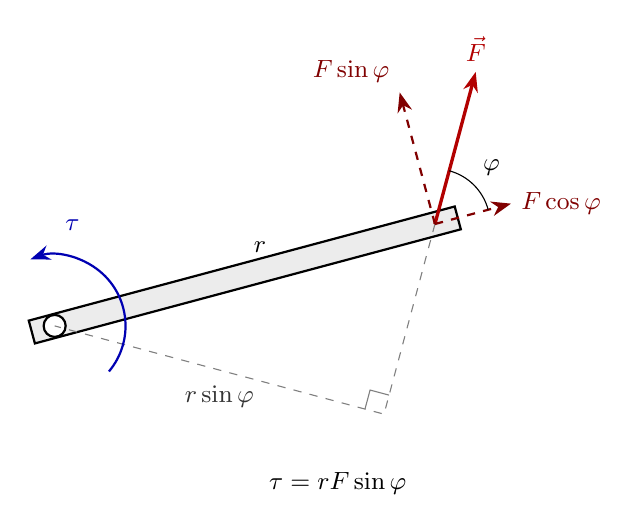
\begin{tikzpicture}[>={Stealth[length=2.5mm]}, every node/.style={font=\small}]
  % Arm along 15 degrees with r = 5; force 2 at 75 degrees (phi = 60): across the arm 2 sin 60 = 1.73, along it 2 cos 60 = 1.
  \coordinate (O) at (0,0);
  \coordinate (P) at (15:5);
  \coordinate (Q) at ($(P)+(15:1)$);
  % Foot of the perpendicular from O to the line of action: P - (r cos phi) u = P + 2.5 (75:-1).
  \coordinate (H) at ($(P)+(75:-2.5)$);
  \draw[thick, fill=gray!15, rotate=15] (-0.3,-0.15) rectangle (5.3,0.15);
  \fill[white, draw=black, thick] (O) circle (0.14);
  \draw[dashed, gray] (P) -- (H) -- (O);
  \draw[gray] ($(H)!0.25cm!(P)$) -- ++(165:0.25) -- ($(H)!0.25cm!(O)$);
  \node[below=2pt, gray!40!black, sloped] at ($(O)!0.5!(H)$) {$r\sin\varphi$};
  \draw[->, very thick, red!70!black] (P) -- ++(75:2) coordinate (F) node[above] {$\vec{F}$};
  \draw[->, thick, dashed, red!50!black] (P) -- ++(105:1.73) node[above left] {$F\sin\varphi$};
  \draw[->, thick, dashed, red!50!black] (P) -- ++(15:1) node[right] {$F\cos\varphi$};
  \pic[draw, "$\varphi$", angle eccentricity=1.45, angle radius=7mm] {angle = Q--P--F};
  \draw[->, thick, blue!70!black] (-40:0.9) arc[start angle=-40, end angle=110, radius=0.9];
  \node[blue!70!black] at (80:1.3) {$\tau$};
  \node[above=3pt] at (15:2.7) {$r$};
  \node[anchor=west] at (2.6,-2) {$\tau = rF\sin\varphi$};
\end{tikzpicture}
